%
% Chapter 12
%

\chapter{RESULTS}
The main purpose of this analysis is to perform a measurment of the best-fit signal strength parameter, known as $\mu$ of the \tth signal process. This parameter
is the factor by which the \tth signal prediction is multiplied to best-fit the observation in data while the backgrounds are constrained
to SM predictions within their systematic uncertainties. An additional measurement that accompanies the measurement of signal strength above
is calculating a 95$\%$ confidence level (CL) upper limit on $\mu$ for the SM \tth process. Both of these measurements quantify the degree to which the signal
and backgrounds are consistent with the observation from data. A description of these methods and the statistical techniques is in the following sections.


\section{Upper Limits}

\begin{table}[htbp]
\begin{center}
  \caption[Table of Final Limits]{95$\%$ CL upper limits on $\mu$ under the background-only hypothesis.}
    \begin{tabular}{c c} \hline
      Observed Limit & Expected Limit $\pm$1$\sigma$  \\ \hline 
      2.9 & 1.0$^{+0.5}_{-0.3}$  \\
      \hline
    \end{tabular}
    \label{tab:limits}
\end{center}
\end{table}

\section{Signal Strength}

\begin{table}[htbp]
\begin{center}
  \caption[Table of best-fit signal strength]{}
    \begin{tabular}{c c c} \hline
      Observed $\mu$ fit $\pm$1$\sigma$ & Expected $\mu$ fit $\pm$1$\sigma$ & Observed(expected) significance & \\ \hline 
      1.7$^{+0.6}_{-0.5}$ & 1.0$^{+0.5}_{-0.5}$ & 3.3$\sigma$ (2.1$\sigma$)  \\
      \hline
    \end{tabular}
    \label{tab:mu}
\end{center}
\end{table}


\begin{table}[htbp]
  \begin{center}
    \caption[Signal region post-fit event yields by lepton flavor]{Expected (post-fit) yields for signal and background processes, and observed yields in data. Yields
      shown after a fit to data with all predictions constrained to SM expectation.}
    \begin{tabular}{l c c c} \hline
      & $\mu\mu$ & $ee$ & $e\mu$  \\ \hline 
      $t\bar{t}W$ & 45.4 $\pm$ 0.5 & 17.8 $\pm$ 0.3 & 64.3 $\pm$ 0.6 \\
      $t\bar{t}Z/\gamma^{*}$ & 16.8 $\pm$ 0.7 & 14.8 $\pm$ 0.8 & 41.7 $\pm$ 1.4 \\
      \hline
      WZ & 5.2 $\pm$ 0.7 & 1.6 $\pm$ 0.4 & 7.5 $\pm$ 0.8 \\
      Rare SM. bkg & 6.8 $\pm$ 0.3 & 3.5 $\pm$ 0.2 & 11.7 $\pm$ 0.4 \\
      WWss & 2.9 $\pm$ 0.2 & 1.4 $\pm$ 0.1 & 4.3 $\pm$ 0.2 \\
      \hline
      Conversions & 0.0 $\pm$ 0.0 & 3.4 $\pm$ 1.1 & 8.5 $\pm$ 1.3 \\
      Charge flip & 0.0 $\pm$ 0.0 & 172 $\pm$ 93 & 149 $\pm$ 82 \\
      Non-prompt leptons & 29.9 $\pm$ 1.2 & 17.3 $\pm$ 1.1 & 53.5 $\pm$ 1.8 \\
      \hline
      Total bkg & 107.3 $\pm$ 1.7 & 70.3 $\pm$ 1.8 & 208.0 $\pm$ 2.9 \\
      \hline
      $t\bar{t}H$ & 18.5 $\pm$ 0.2 & 7.4 $\pm$ 0.1 & 26.2 $\pm$ 0.2 \\
      \hline
      Data & 154 & 95 & 274 \\
      \hline
    \end{tabular}
    \label{tab:yields}
  \end{center}
\end{table}


\begin{figure}[htb]
        \centering 
        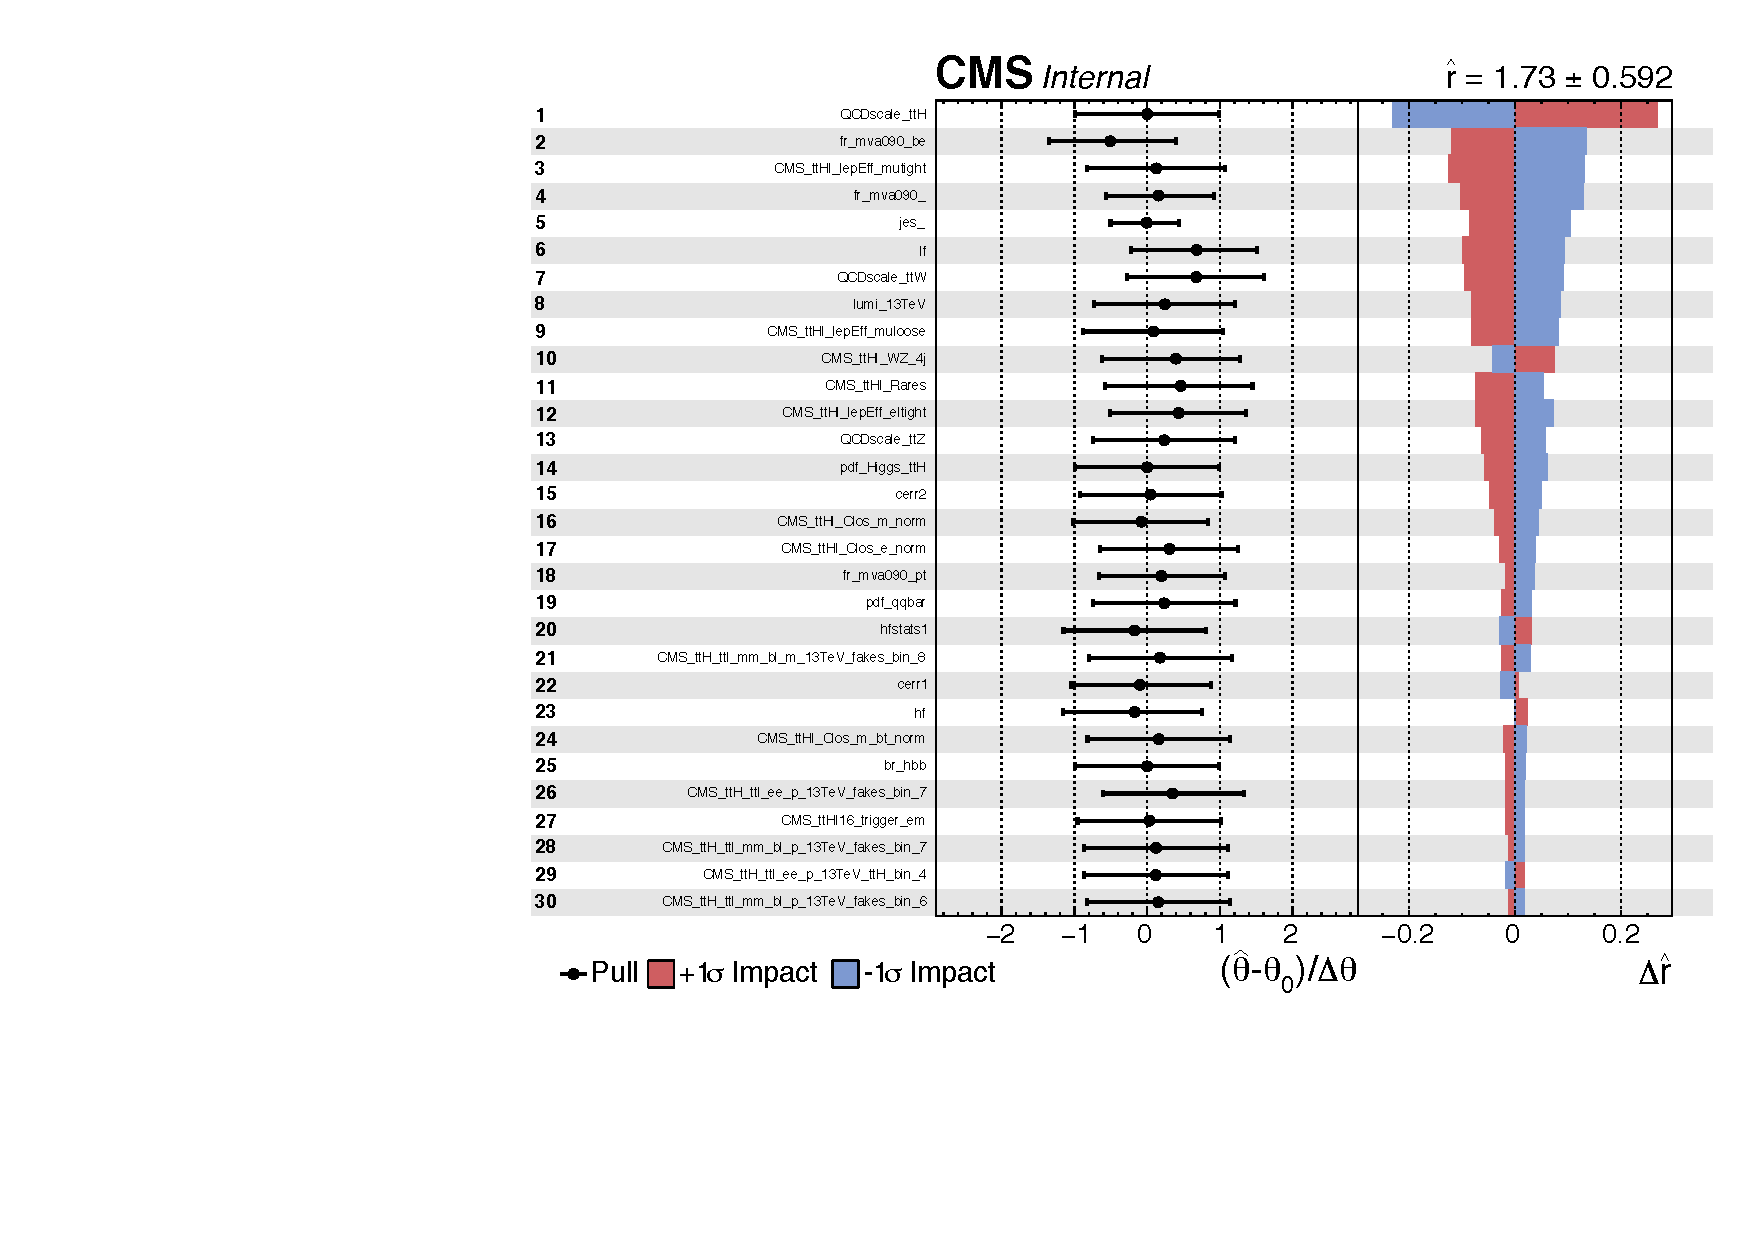
\includegraphics[width=0.95\textwidth]{ch11_figs/impacts_ttH_13TeV_top30.pdf}
        \caption[Nuisance parameter impacts]{The top nuisance parameters ranked by their impact on the fit. The pull of each nuisance (left) is the amount by which the fit moves that parameter from its
        initial value. The impact of each nuisance (right) is the change in best-fit $\mu$ divided by the uncertainty in $\mu$, obtained by moving each nuisance up (red) or down (blue) by 1$\sigma$.}
        \label{fig:impacts}
\end{figure}



\section{Conclusion}

%% \begin{figure}[hbtp]
%%  \begin{center}
%%    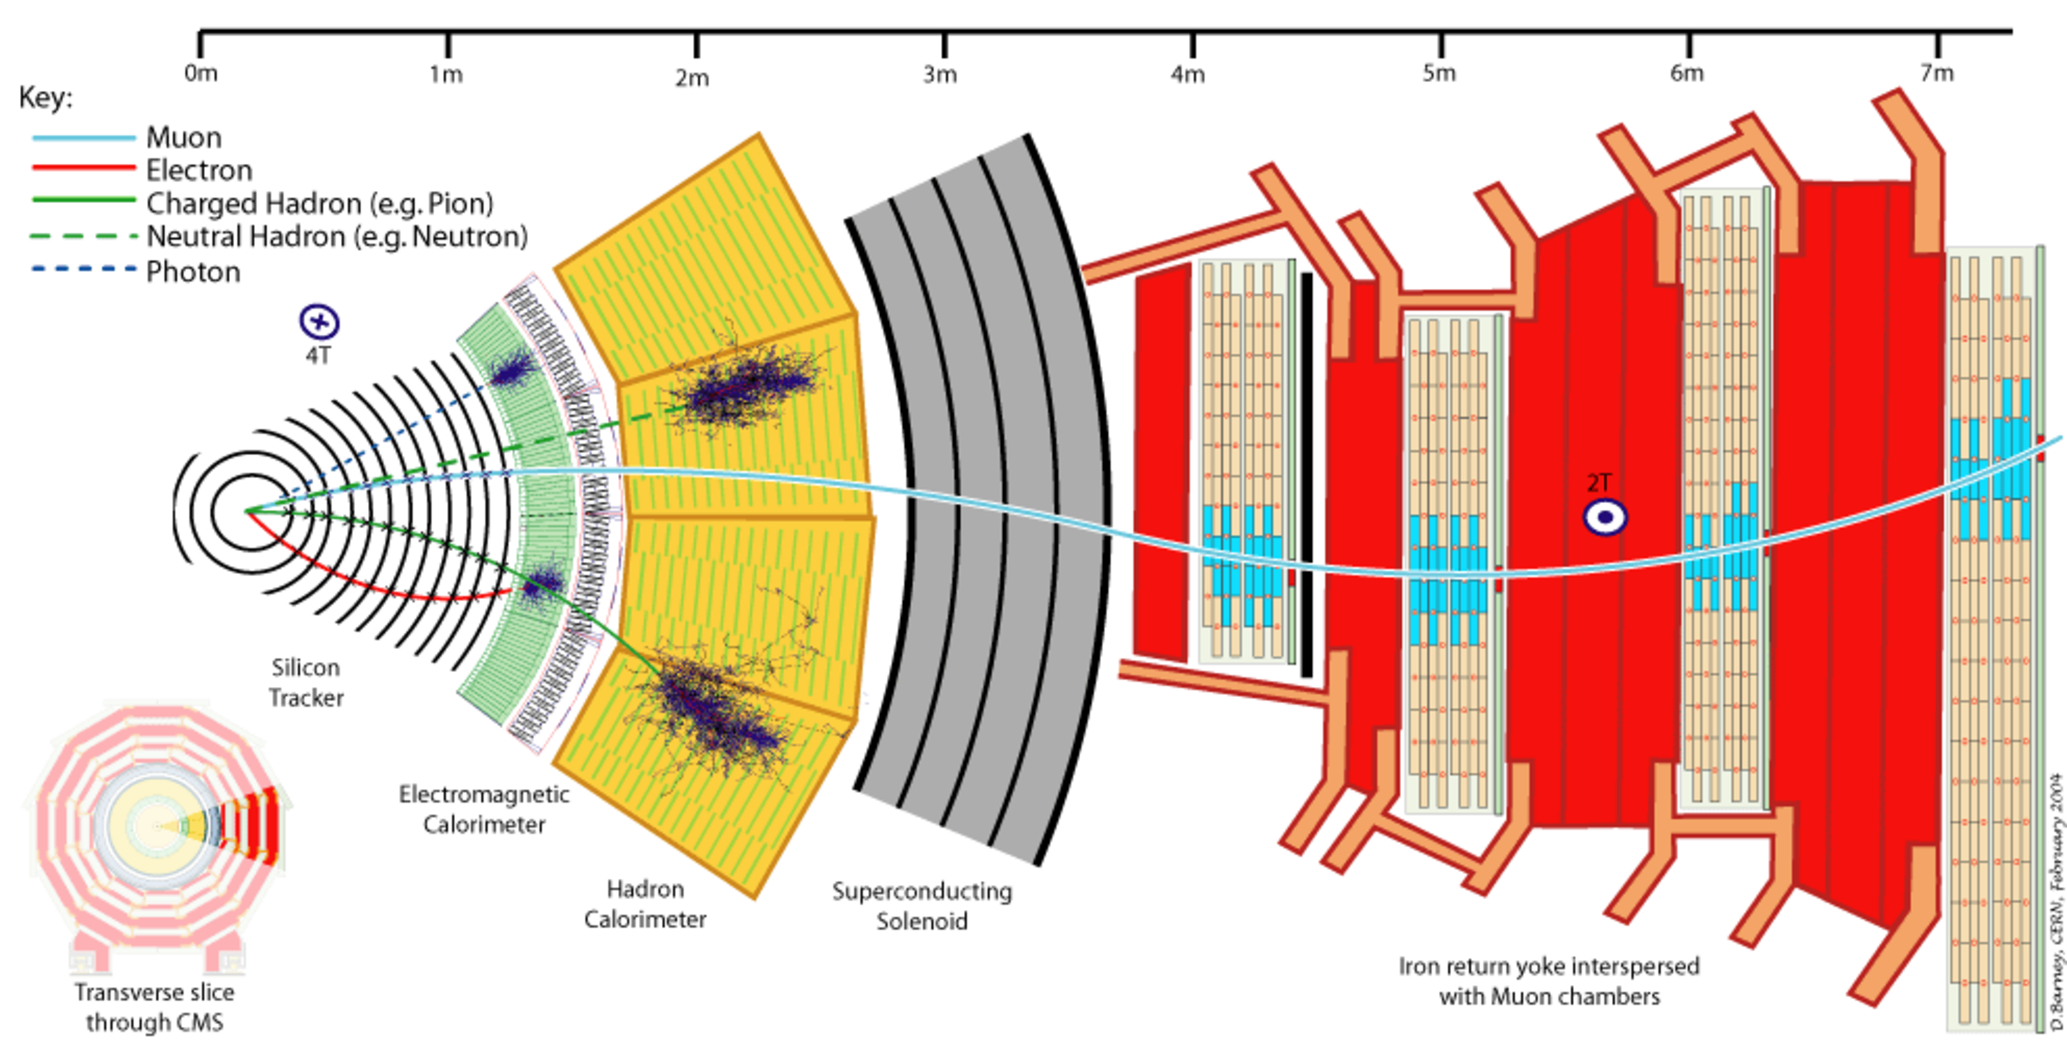
\includegraphics[width=0.8\textwidth]{ch4_figs/cms_particleflow.pdf}
%%    \caption{An overview of how CMS detects different types of particles. The slice of CMS in in the x-y plane.~\cite{NEED CITATION}.}
%%    \label{fig:cms_pflow}
%%  \end{center}
%% \end{figure}
